\documentclass[report/main.tex]{subfiles}

% A description and illustration of:

% - How do you interact as developers?
% - How is the team organized?
% - A complete description of stages and tools included in the CI/CD chains.
%     - That is, including deployment and release of your systems.
% - Organization of your repositor(ies).
%     - That is, either the structure of of mono-repository or organization of artifacts across repositories.
%     - In essence, it has to be be clear what is stored where and why.
% - Applied branching strategy.
% - Applied development process and tools supporting it
%     - For example, how did you use issues, Kanban boards, etc. to organize open tasks
% - How do you monitor your systems and what precisely do you monitor?
% - What do you log in your systems and how do you aggregate logs?
% - Brief results of the security assessment.
% - Applied strategy for scaling and load balancing.

% In essence it has to be clear how code or other artifacts come from idea into the running system and everything that happens on the way.

\begin{document}
    \section{Process' Perspective}
    \label{Sec:process_perspective}
        \subsection{Development Team}
        \label{subsec:development-team}
            To adopt a DevOps organisation and develop style as specified in \cite{devops-handbook} part 1, a mix of various software development strategies and frameworks was chosen, support by tools to support these strategies. In this section the development strategies will be covered first followed by the tools used.
            
            \subsubsection{Development Strategies}
            \label{subsubsec:development-strategies}
                % self organising teams?
                To accommodate the DevOps principles of 'smaller batch sizes' and 'Reduce the number of handoffs' (\cite{devops-handbook} p. 9-10), an agile approach was taken to the development by using the agile principle of "Deliver working software frequently ..." (\cite{agile-manifesto-second-page} para. 5). This lead to a delivery interval of 1 week with a release on Sunday evening marking the end of an interval.
                
                Team members had other commitments which made it hard to find common working hours, hence a self organising approach was chosen (\cite{agile-manifesto-second-page} para. 13) to handle this issue. With this short overlapping working time, it was decided to practice the Scrum daily meetings (\cite{2020-scrum-guide} p. 9) two times per week, one on Mondays and one Thursdays. The Monday meetings would be used for prioritising and planning, while Thursday meetings were more of a catch up and experience exchange.
                
                Various tools was utilised to achieve the above strategies, which will be covered in the next sections.
                
                %Each meeting started with stand up meeting where everyone summarised what have been achieved since the session and what we expect to be done until next week. On Mondays we defined the task that we plan to do on the given with priorities assigned to each of them. Also, we picked the individual or group tasks for the week through out the week the individuals and groups work on the tasks in a self-organising manner. The Thursday session had the main focus demonstrating the progress ,helping each other out if one of the group or group member is stuck with a task and deciding on the which task to pick if we were done with the one picked on Monday.
        
        \subsection{Development Tools}
        \label{subsec:development-tools}
            \subsubsection{Communication Tools}
            \label{subsubsec:communication-tools}
                Communication and meetings between team members were done by using a Team Group. The Group contained 3 channels a general chat, a chat for arranging meetings/hosting meetings and a chat that contains various useful links. %This enabled us ask questions and provide feed back out side of the meetings, thus we could work on the project more continuously. We organised the tasks in Kanban, this way we could easily track the progression of them and see which ones need to be worked on urgently.
                
            \subsubsection{Planning tools}
            \label{subsubsec:planning-tools}
                A Kanban board was create with Github Projects\footnote{TODO} in combination with Github Issues\footnote{TODO} as the sticky notes in it to keep an overview of the tasks at hand. Issues could be added to the project in two ways. Every Monday once the tasks for the following week was known, issues would be created and added to the project. They would then be prioritised in regards to the severity for the application i.e. security risks would be handled as quickly as possible while minor UI bugs would be fixed last. If any bugs became apparent at any point they could be added to the project, where after the developers would assess severity as soon as possible. All of this can be seen in figure \ref{fig:kanban-board-1}  together with part of the column setup, which can be seen below
                
                \begin{center}
                    To Do $\longrightarrow$ In Progress $\longrightarrow$ Review In Progress $\longrightarrow$ Done $\longrightarrow$ Deployed $\longrightarrow$ To Be Archived
                \end{center}
                
                \begin{figure}[H]
                    \centering
                    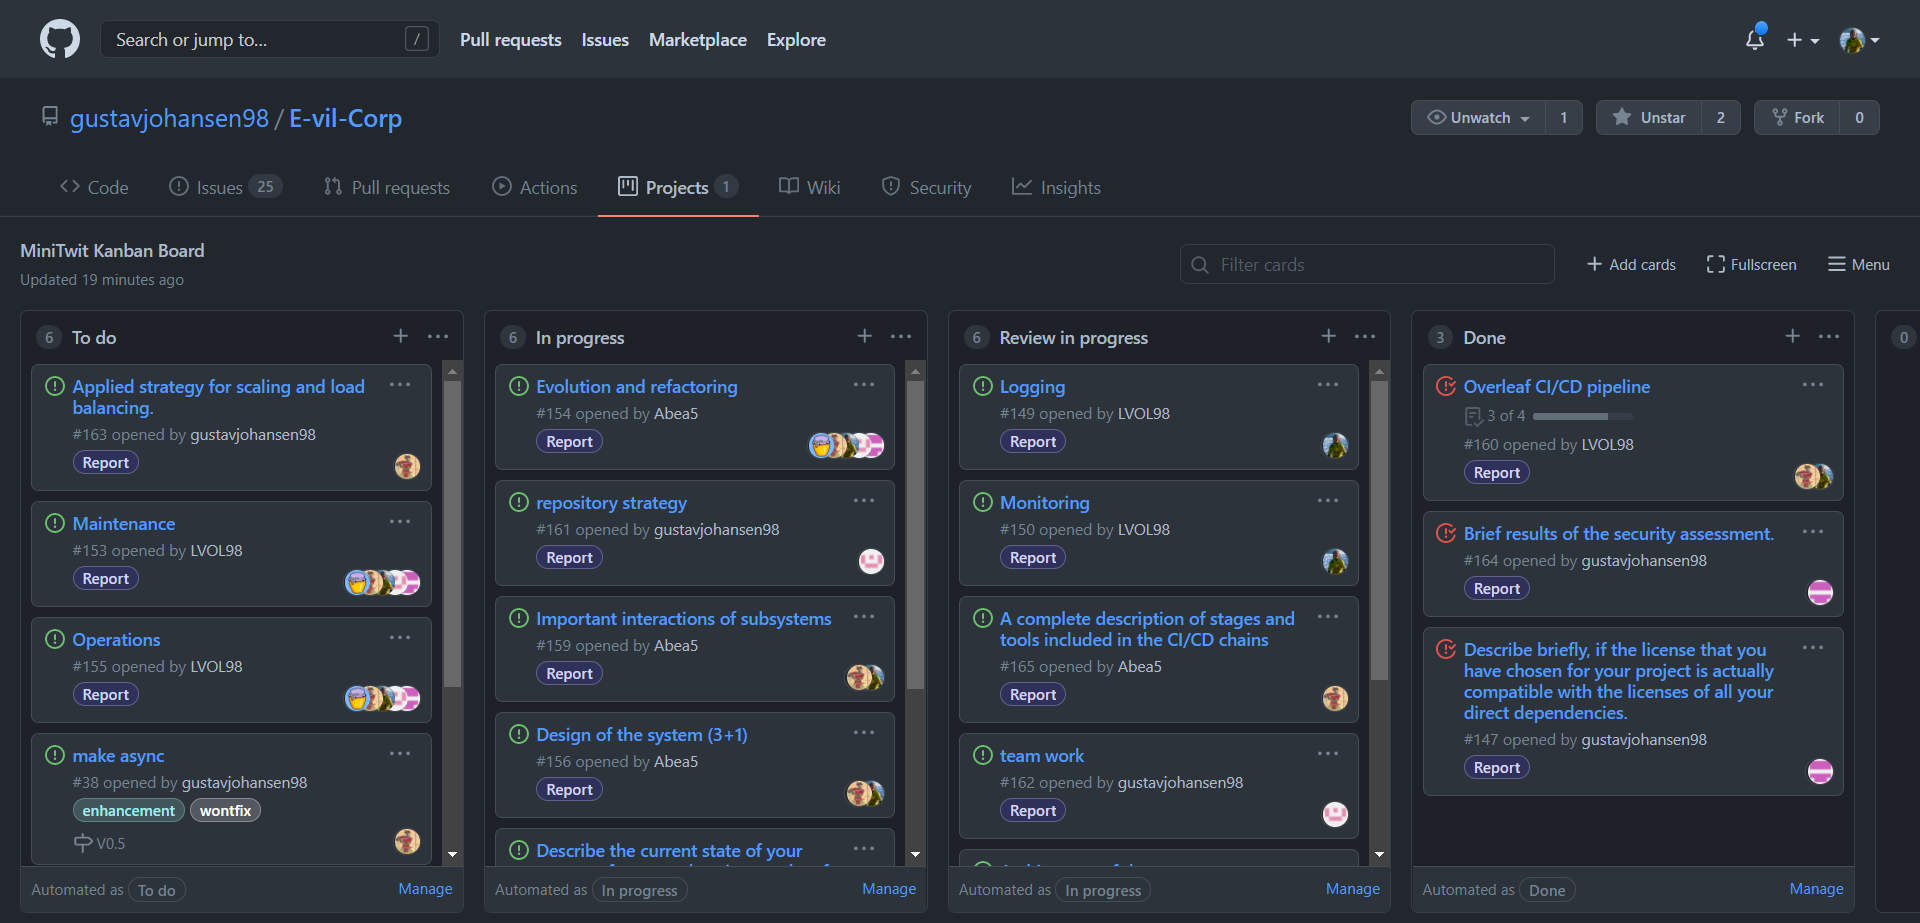
\includegraphics[width=0.8\textwidth]{report/images/Kanban board 1.png}
                    \caption{TODO}
                    \label{fig:kanban-board-1}
                \end{figure}

            \subsubsection{Version Control}
            \label{subsubsec:version-control}
                % TODO: Specify folders in repo?!?!
                Git was used as the version control system and Github was used to host the repositories. A mono-repository setup as utilised to host the source code, with a task based branching strategy (\cite{task-branching}) combined with a develop and main branch. Meaning that main contained code that was deployed and develop was a branch for testing and merging the different task branches.
                %We used  repository. We developed on our local machines and pushed to the development branch first. The have been deployed when it was pushed to the main branch. Before merging the development branch with the main, at least two group members reviewed the code and tested the new functionality.
                
        \subsection{Monitoring}
        \label{SubSec:monitoring}
            % - How do you monitor your systems and what precisely do you monitor?
            The monitoring of the EvilTwitter application was done using the monitoring and alerting toolkit Prometheus\footnote{\hyperlink{https://prometheus.io/}{https://prometheus.io/}} to gather information from the application. Two dotnet package was used to retrieve data from the application. Prometheus-net.SystemMetrics\footnote{\hyperlink{https://github.com/Daniel15/prometheus-net.SystemMetrics}{https://github.com/Daniel15/prometheus-net.SystemMetrics}} was used to retreive system information from where the application was running, and prometheus-net\footnote{\hyperlink{https://github.com/prometheus-net/prometheus-net}{https://github.com/prometheus-net/prometheus-net}} to gather information from the Controllers. The application posted all the collected data at \textit{http://159.89.213.38:5010/metrics} where Prometheus could then gather the necessary data.
                
            Prometheus then made its services available at \textit{http://159.89.213.38:9090} where Grafana\footnote{\hyperlink{https://grafana.com/}{https://grafana.com/}} could connect and retrieve the necessary data. Via grafana this data was changed to a more readable format collected in a dashboard that was made available at \textit{http://159.89.213.38:3000}.
            
            The information gathered in Grafana was setup in two categories: General and controller usage
                
            \begin{figure}[H]
                \centering
                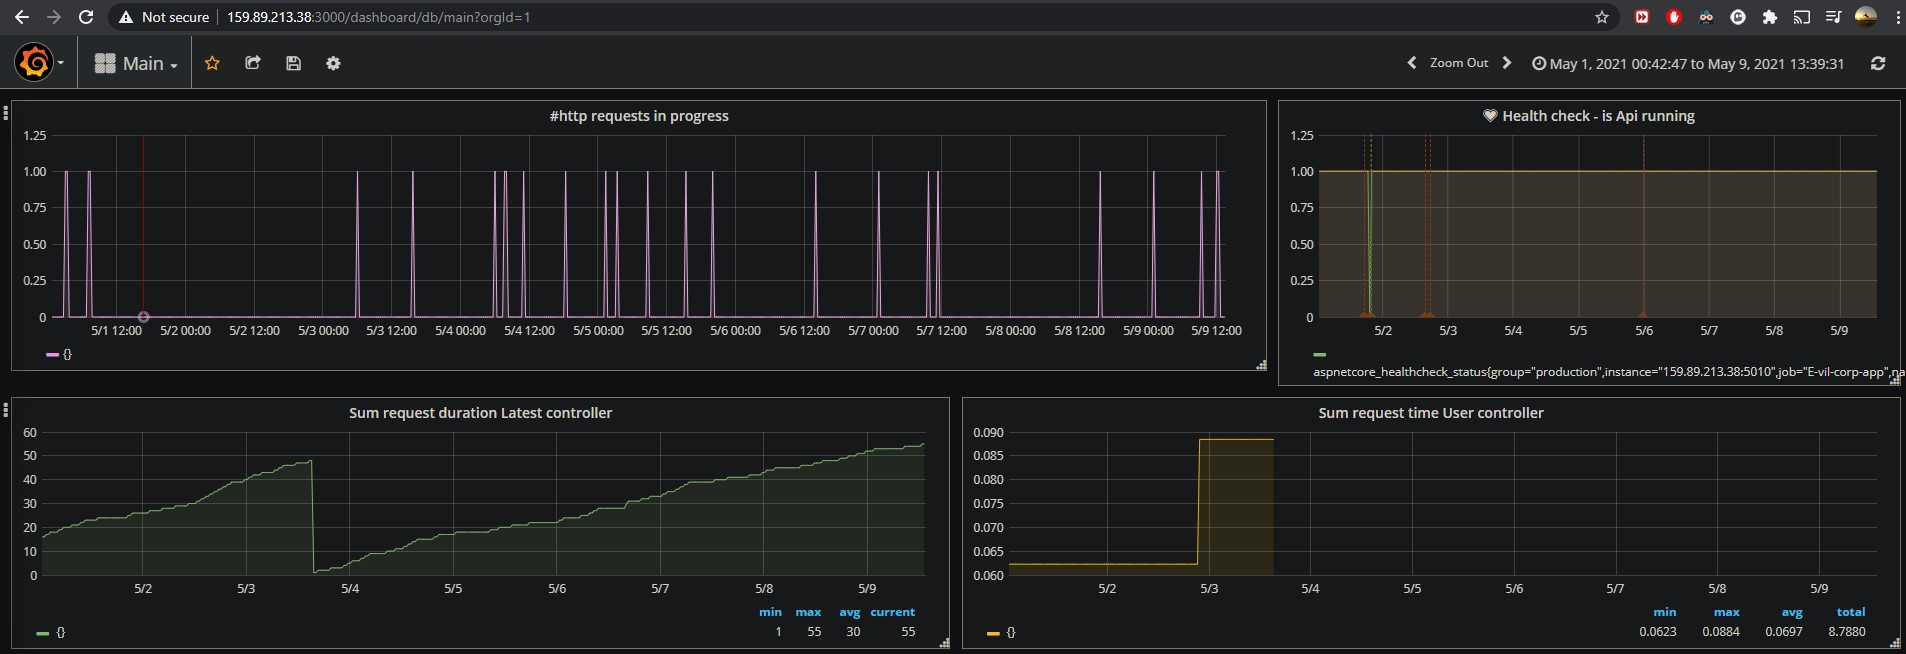
\includegraphics[width=\textwidth]{report/images/Grafana EvilTwitter 1.jpg}
                \caption{TODO}
                \label{fig:grafana_setup_1}
            \end{figure}
                
            \begin{figure}[H]
                \centering
                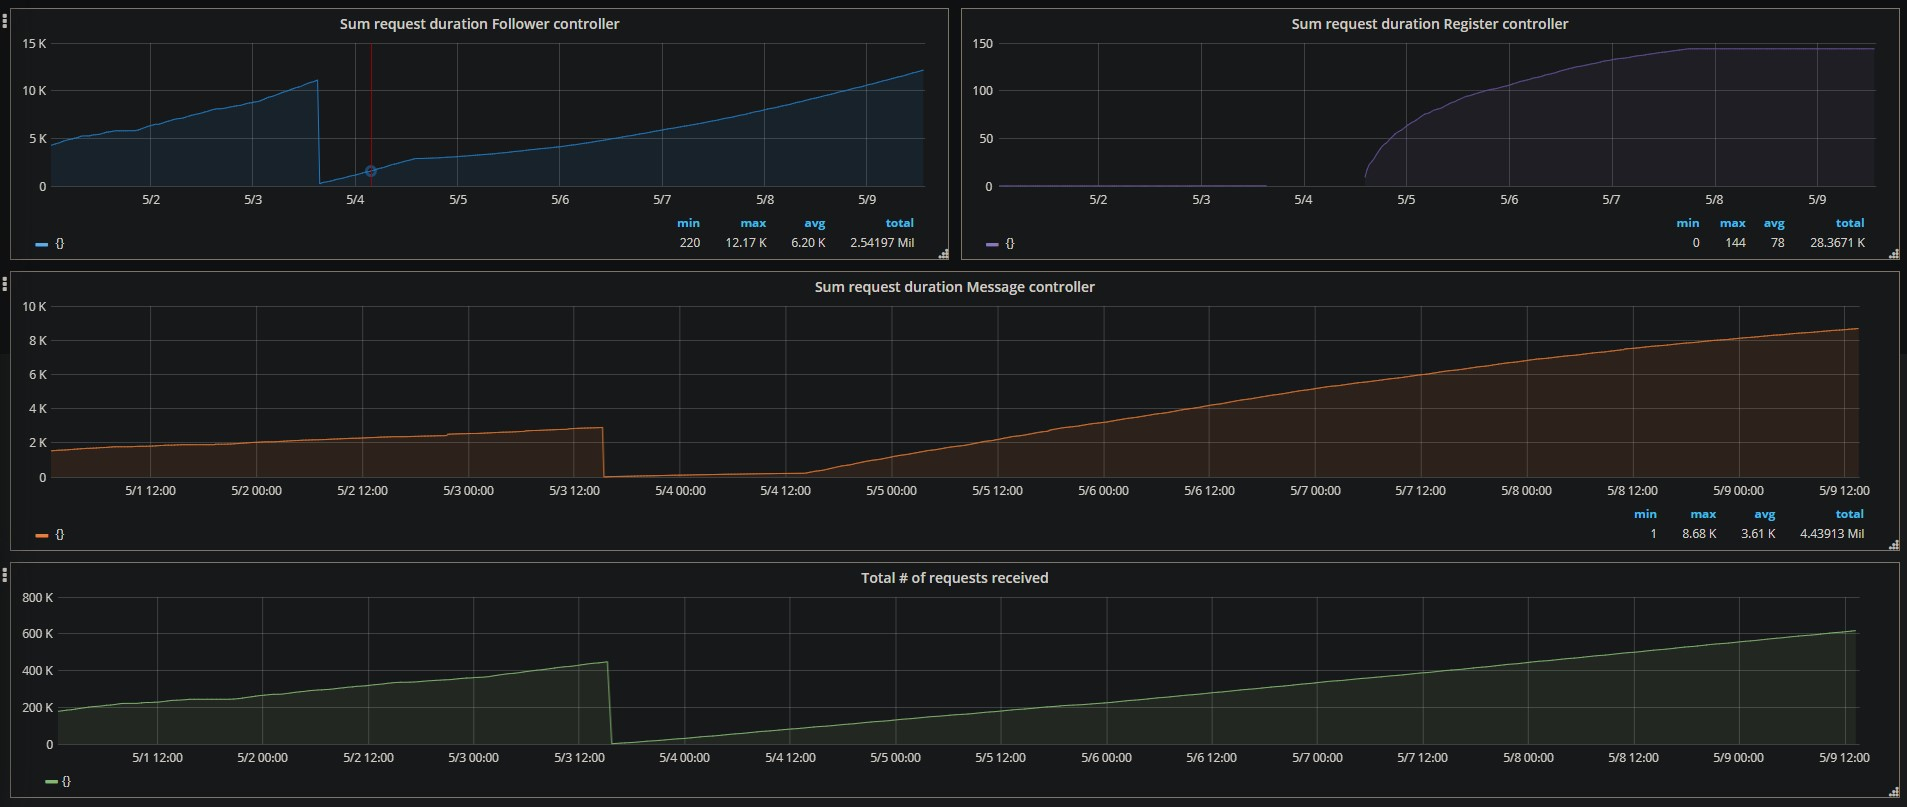
\includegraphics[width=\textwidth]{report/images/Grafana EvilTwitter 2.jpg}
                \caption{TODO}
                \label{fig:grafana_setup_2}
            \end{figure}
            
            First at the top row of figure \ref{fig:grafana_setup_1} the genral view of the application is given. This includes a graph over how many request is occurring at a given time (the graph to the left), to give an overview of the incoming traffic. Further, the alert graph can be seen at the top right, which is a value that can be either 1 or 0. This translates to what value latest returned last, with any latest value greater than 0 would resolved to a value of 1 and anything else would resolved to a value of 0. Hence if the Api is down or returns odd values this would be registered by Grafana. This tracker could be used to notify the developers if the Api behaved oddly, which was utilised by having a webhook that sends messages to a discord server as seen in the figure \ref{fig:grafana_discord_alert}.
                
            \begin{figure}[H]
                \centering
                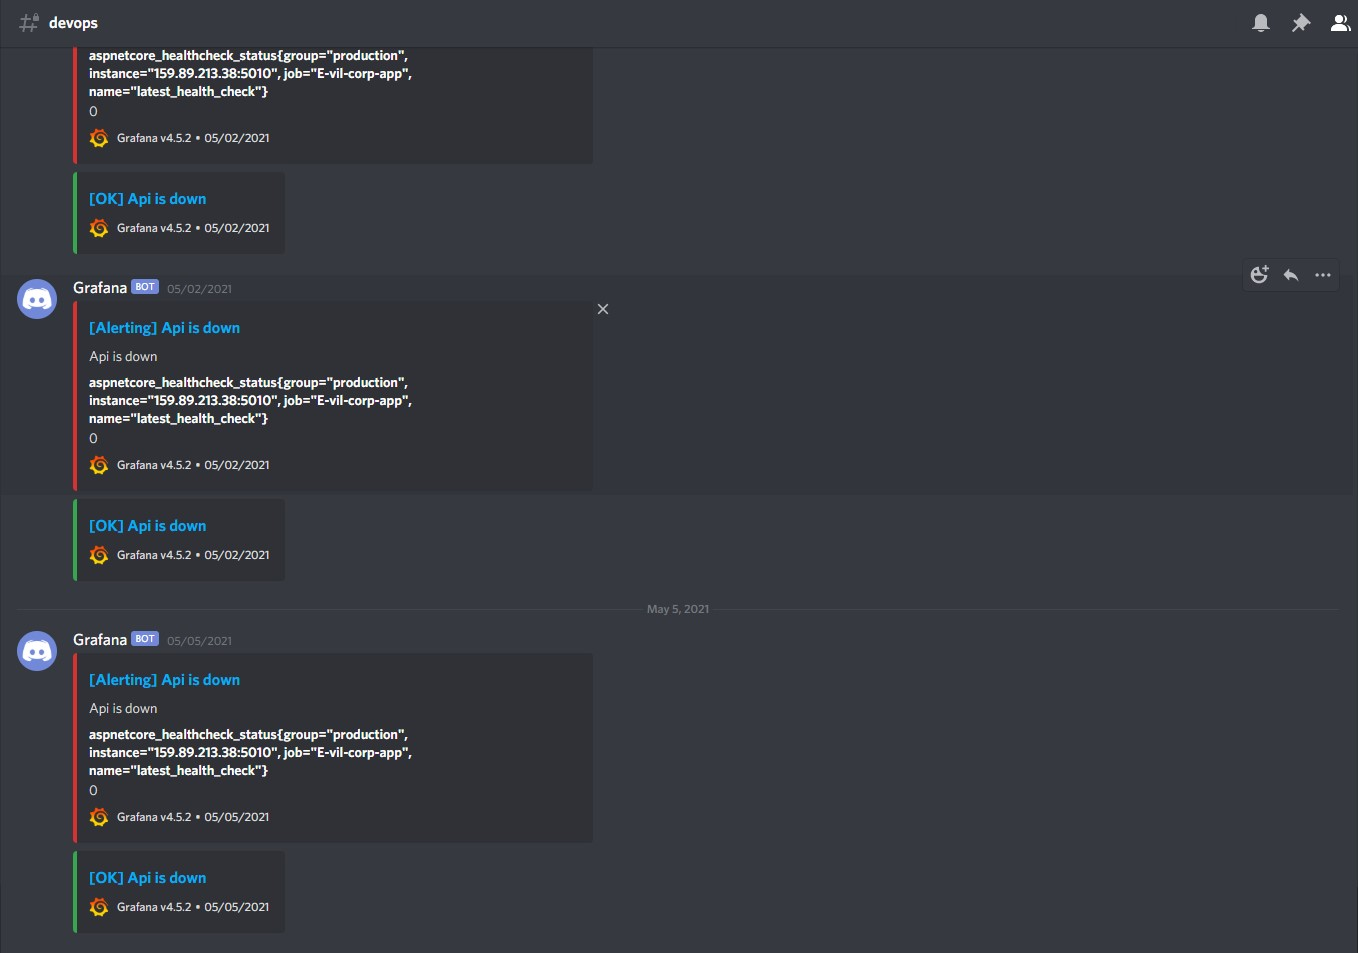
\includegraphics[width=\textwidth]{report/images/Grafana Discord Alert.jpg}
                \caption{TODO}
                \label{fig:grafana_discord_alert}
            \end{figure}
            
            % TODO: the shortened or the longer version?!?!
            Second information from controllers was very detailed\footnote{The data posted can be seen at \hyperlink{http://159.89.213.38:5010/metrics}{http://159.89.213.38:5010/metrics}}, and could be filtered by message type (POST, GET etc), response (204, 404 etc.). This information is valuable in solving performance issues, but creating a graph for every single message type and response would clutter the dashboard and make it less readable. Hence a decision was made that such queries should be done on a case by case basis, and a more general overview was created to monitor each controller as a whole. The query can be seen below.
                
            \begin{center}
                sum(http\_request\_duration\_seconds\_sum{controller="Follower"})
            \end{center}
                
            Everything else on the Grafana dashboard is the query above executed on all controllers. An example to the use fullness of this approach can be seen in the following example. At one point the message controller was more time as the other controllers, where by looking on the summarised time per message type revealed that it was the GET call that used a lot of time.
                

        \subsection{Logging}
            \label{SubSec:logging}
            % - What do you log in your systems and how do you aggregate logs?
            The application uses Elastic Search\footnote{TODO}, Kibana\footnote{TODO} and Serilog\footnote{TODO} to aggregate the logs. This is done by having C\# logs useful information that is then propagated to \textit{http://localhost:9200} where Elastic Search monitors and collects log. Finally Kibana imports this data in order to display and query the logs.
            
            The package Serilog came with some off the shelf functionality in case of logging, where at the informational level the following functionality was utilised initially. Logging of database queries and requests and response send to and from the controllers. After evaluation this was deemed unnecessary, as the information given in the logs could be retrieved wither from the monitoring setup or from database queries themselves, hence logging was kept at an error level as this information cannot be retrieved otherwise.

        \subsection{Security assessment}
        To assess the security of our system, we considered vulnerabilities of our cloud infrastructure, vulnerabilities of the code we produced, and security of the user data.
        When assessing the safety of our infrastructure, we found it high impact and high probability that an adversary gains access to the account of the repo owner, gaining access to our secrets. To decrease this risk, the repo owner enabled 2-factor authentication. We also found it high probability high impact to fall victim to a denial-of-service attack, since DoS attacks are cheap to execute, and we have no protection set up against it. The system could also be overwhelmed by automated sign-ups to the platform, so it would be advantageous to set up CAPTCHA against it.
        
        Considering we use the insecure version of http, our users are at risk of an adversary eavesdropping or spoofing our server's IP. This in turn would lead to disclosure of the user's credentials. Could by remedied by self-signing a certificate with Let's Encrypt. We deemed this issue medium impact and medium probability.
        
        One low probability risk we identified was the cloud provider (or our account at the provider) getting hacked. This would be a severe problem, since we would lose access to our infrastructure, with the adversary gaining complete control over the live server and our database. User credentials would be somewhat safe, we only store hashes of passwords, however common passwords could be easily looked up from a rainbow table. To provide better guarantees, we could also add salt and pepper to the passwords.
        The other low probability risk we identified was a supply chain attack on any of our dependencies. Since it is unfeasible to constantly audit every new version the supplier publishes, the best line of defence is auditing once, and freezing version numbers after.
        
        \subsection{Description of CI/CD pipeline}
        Overall, the project consists of three workflows all utilised with GitHub Actions to make use of the open source workflow actions found in the GitHub Marketplace:
        \begin{itemize} 
            \item \textbf{release.yml} to automatically make a release every Sunday at 9 pm. 
            \item \textbf{report-overleaf.yml} to automatically compile the Latex source code into a pdf.
            \item \textbf{main.yml} to deploy local changes from development to production.
        \end{itemize}
        
        All the workflow files are found in the \textit{.github/workflows} folder of the repository, and each uses the action checkout\footnote{\hyperlink{checkout action}{https://github.com/actions/checkout}} to checkout the repository to a virtual machine hosted by GitHub to perform operations on. 
        
        \subsubsection{Automatic release}
        
        This workflow uses the create-release\footnote{\hyperlink{release action}{https://github.com/actions/create-release}} and CRON formatting to automatically trigger a release of the main branch every sunday at 9 pm. 
        
        \subsubsection{Latex report build}
        
        We write the report in Overleaf and from their platform, we push the changes in the Latex documents directly to main, which compiles them to a pdf via the latex-action\footnote{\hyperlink{latex compiler action}{https://github.com/xu-cheng/latex-action}}. We then use the push action\footnote{\hyperlink{push action}{https://github.com/ad-m/github-push-action}} to push the pdf document back into the correct folder in the repository. 
        
        
        \subsubsection{From development to production}
        
        \begin{figure}[H]
            \centering
                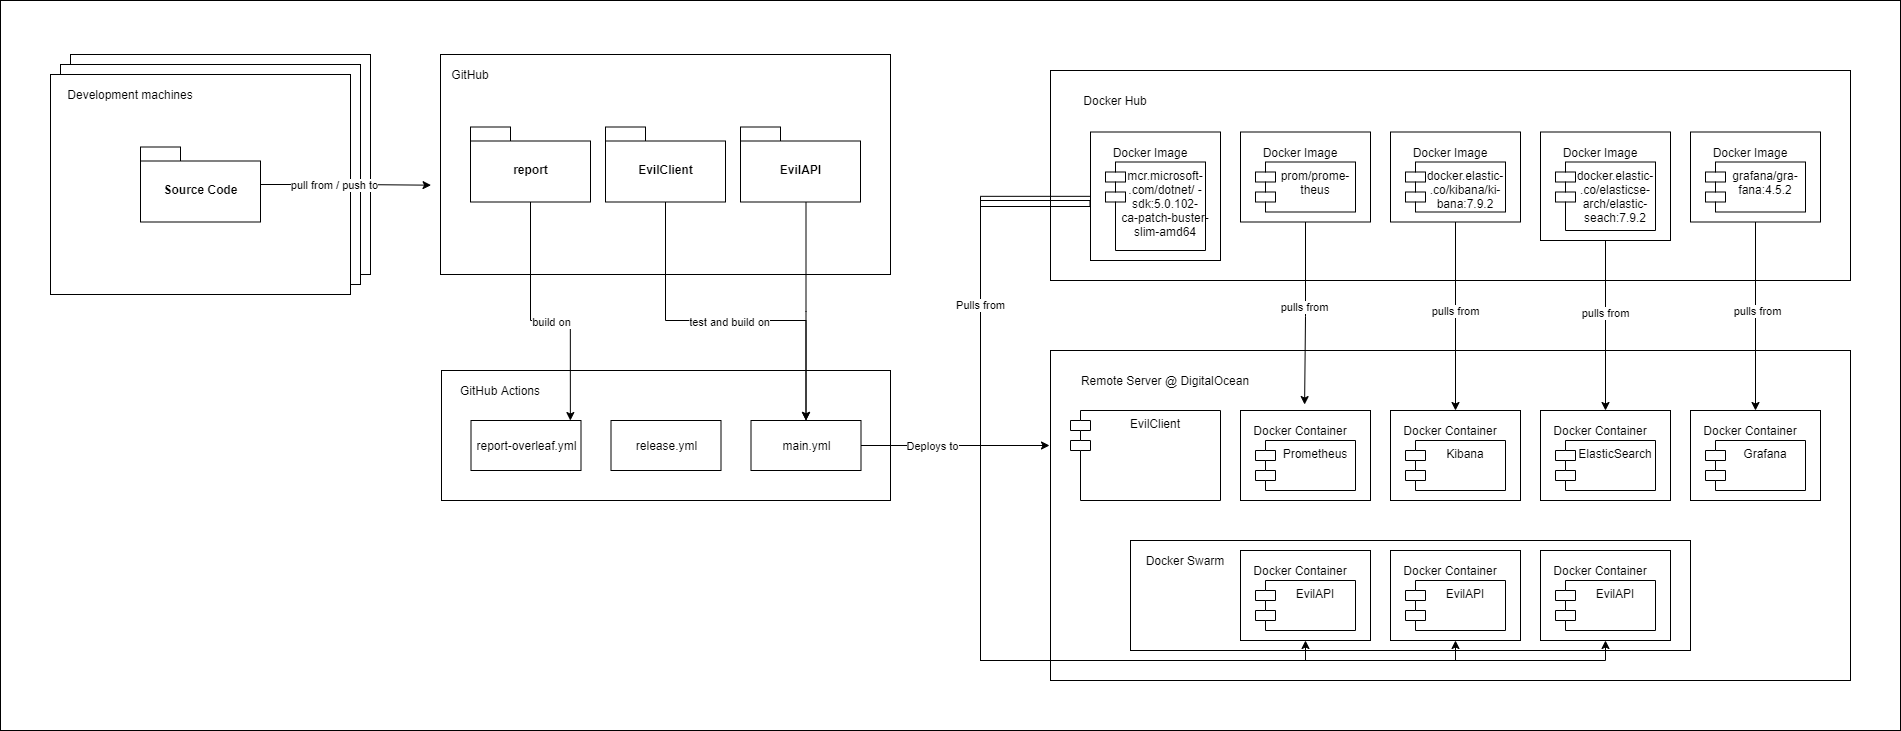
\includegraphics[width=\textwidth]{report/images/MiniTwit-workflow-final.png}
                \caption{Overall workflow diagram}
            \label{fig:overall_workflow}
        \end{figure}
        
        Figure 4 displays the different stages on how implementations are taken from development into production. We can make use of a tier structure to explain the details:
        
        \begin{enumerate}
            \item \textbf{Development tier} \\
            Changes to the source code are made in this tier on individual developer workstations. To ensure code quality before pushing to version control, the project uses the dotnet CodeCracker\footnote{\hyperlink{CodeCracker}{https://github.com/code-cracker/code-cracker}} package to provide the developer with a static code analysis when building locally. 
            
            \item \textbf{Integration tier} \\
            Upon merging into the main branch, the \textit{main.yml} workflow will be triggered. This workflow handles testing, quality control and staging and is separated into three jobs, that will run on GitHub Actions hosted containers: 
            
            \begin{itemize}
                \item \textbf{Build, test and Infersharp analysis} \\
                This job runs in an Ubuntu 18.04 environment to resemble the actual target production environment hence staging. Here, dependencies are restored, the source code will be built and all the unit tests will be performed. Furthermore, we make use of the Infersharp action\footnote{\hyperlink{Infersharp action}{https://github.com/microsoft/infersharpaction}}, that will detect security leaks such as exposed connectionstrings for instance.  
                
                \item \textbf{Build and SonarCloud analysis} \\
                The second job runs in a Windows latest version environment, since the SonarCloud static code analysis depends on this environment. When built and completed, a comprehensive code analysis is available on our SonarCloud dashboard. 
                
            \end{itemize}
            
            Both of these jobs run concurrently and utilise the dotnet action\footnote{\hyperlink{dotnet action}{https://github.com/actions/setup-dotnet}} with dotnet version 5.0.102 to mirror the dotnet environment in production. 
            
            
            \item \textbf{Deployment tier} \\
            The third job of the \textit{main.yml} workflow handles continuous deployment and is dependent on the aforementioned jobs, as shown in figure 5. 
            
            \begin{figure}[H]
            \centering
                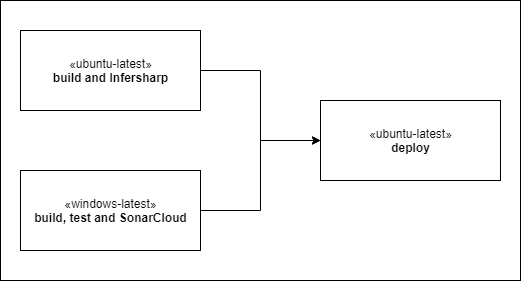
\includegraphics[width=\textwidth/2]{report/images/MiniTwit-main-final.png}
                \caption{Main Workflow diagram}
            \label{fig:main_workflow}
            \end{figure}
            
            That is, this final job will be triggered if and only if the other jobs succeed, and upon success the job will run the deployment script:
            
            \begin{itemize}
                \item Checkout the repository from main. 
                \item Copy repository to DigitalOcean droplet via SCP action\footnote{\hyperlink{scp action}{https://github.com/appleboy/scp-action}}. 
                \item SSH into the droplet via SSH action\footnote{\hyperlink{ssh action}{https://github.com/appleboy/ssh-action}}.
                \item Run the swarm deploy script, such that the api docker service updates its running containers with the latest build of the EvilAPI subsystem. 
                \item Run an instance of the EvilClient subsystem. 
                \item Run the Grafana, Kibana, ElasticSearch and Prometheus containers if they are not already running via docker-compose.  
            \end{itemize}
            
            If the rolling update in the api docker service fails, an automatic rollback to the previous image will be performed. Unfortunately, the EvilClient instance does not have any rollback strategy upon failures as of now.  
            
        \end{enumerate}
        
        
        \subsection{Applied strategy for scaling and load balancing}
        
        
            
\end{document}